\jxhj{%教学后记
	}
\skrq{%授课日期
	2017年5月13日 4-5节}
\ktmq{%课题名称
	 变量周边倒圆角}
\jxmb{%教学目标,每行前面要加 \item
	\item 掌握简单零件的倒圆;
	\item 掌握相关数学处理;
	\item 掌握循环的几个特点;
	\item 掌握简单零件的倒角。}
\jxzd{%教学重点,每行前面要加 \item
	\item 掌握简单零件的倒圆;
	\item 掌握简单零件的倒角。}
\jxnd{%教学难点,每行前面要加 \item
	\item 相关数学处理。}
\jjff{%教学方法
	通过讲述、举例、演示法来说明;}

\makeshouye %制作教案首页

%%%%教学内容
\subsection{组织教学}
\begin{enumerate}[\hspace{2em}1、]
	\item 集中学生注意力;
	\item 清查学生人数;
	\item 维持课堂纪律;
\end{enumerate}
\subsection{复习导入及主要内容}
\begin{enumerate}[1、]
	\item 加工轮廓的处理;
	\item 极坐标;
	\item 加工工序。
\end{enumerate}


\subsection{教学内容及过程}

\subsubsection{简单零件的倒角}
如图\ref{园锥}所示:
\begin{figure}
	\centering	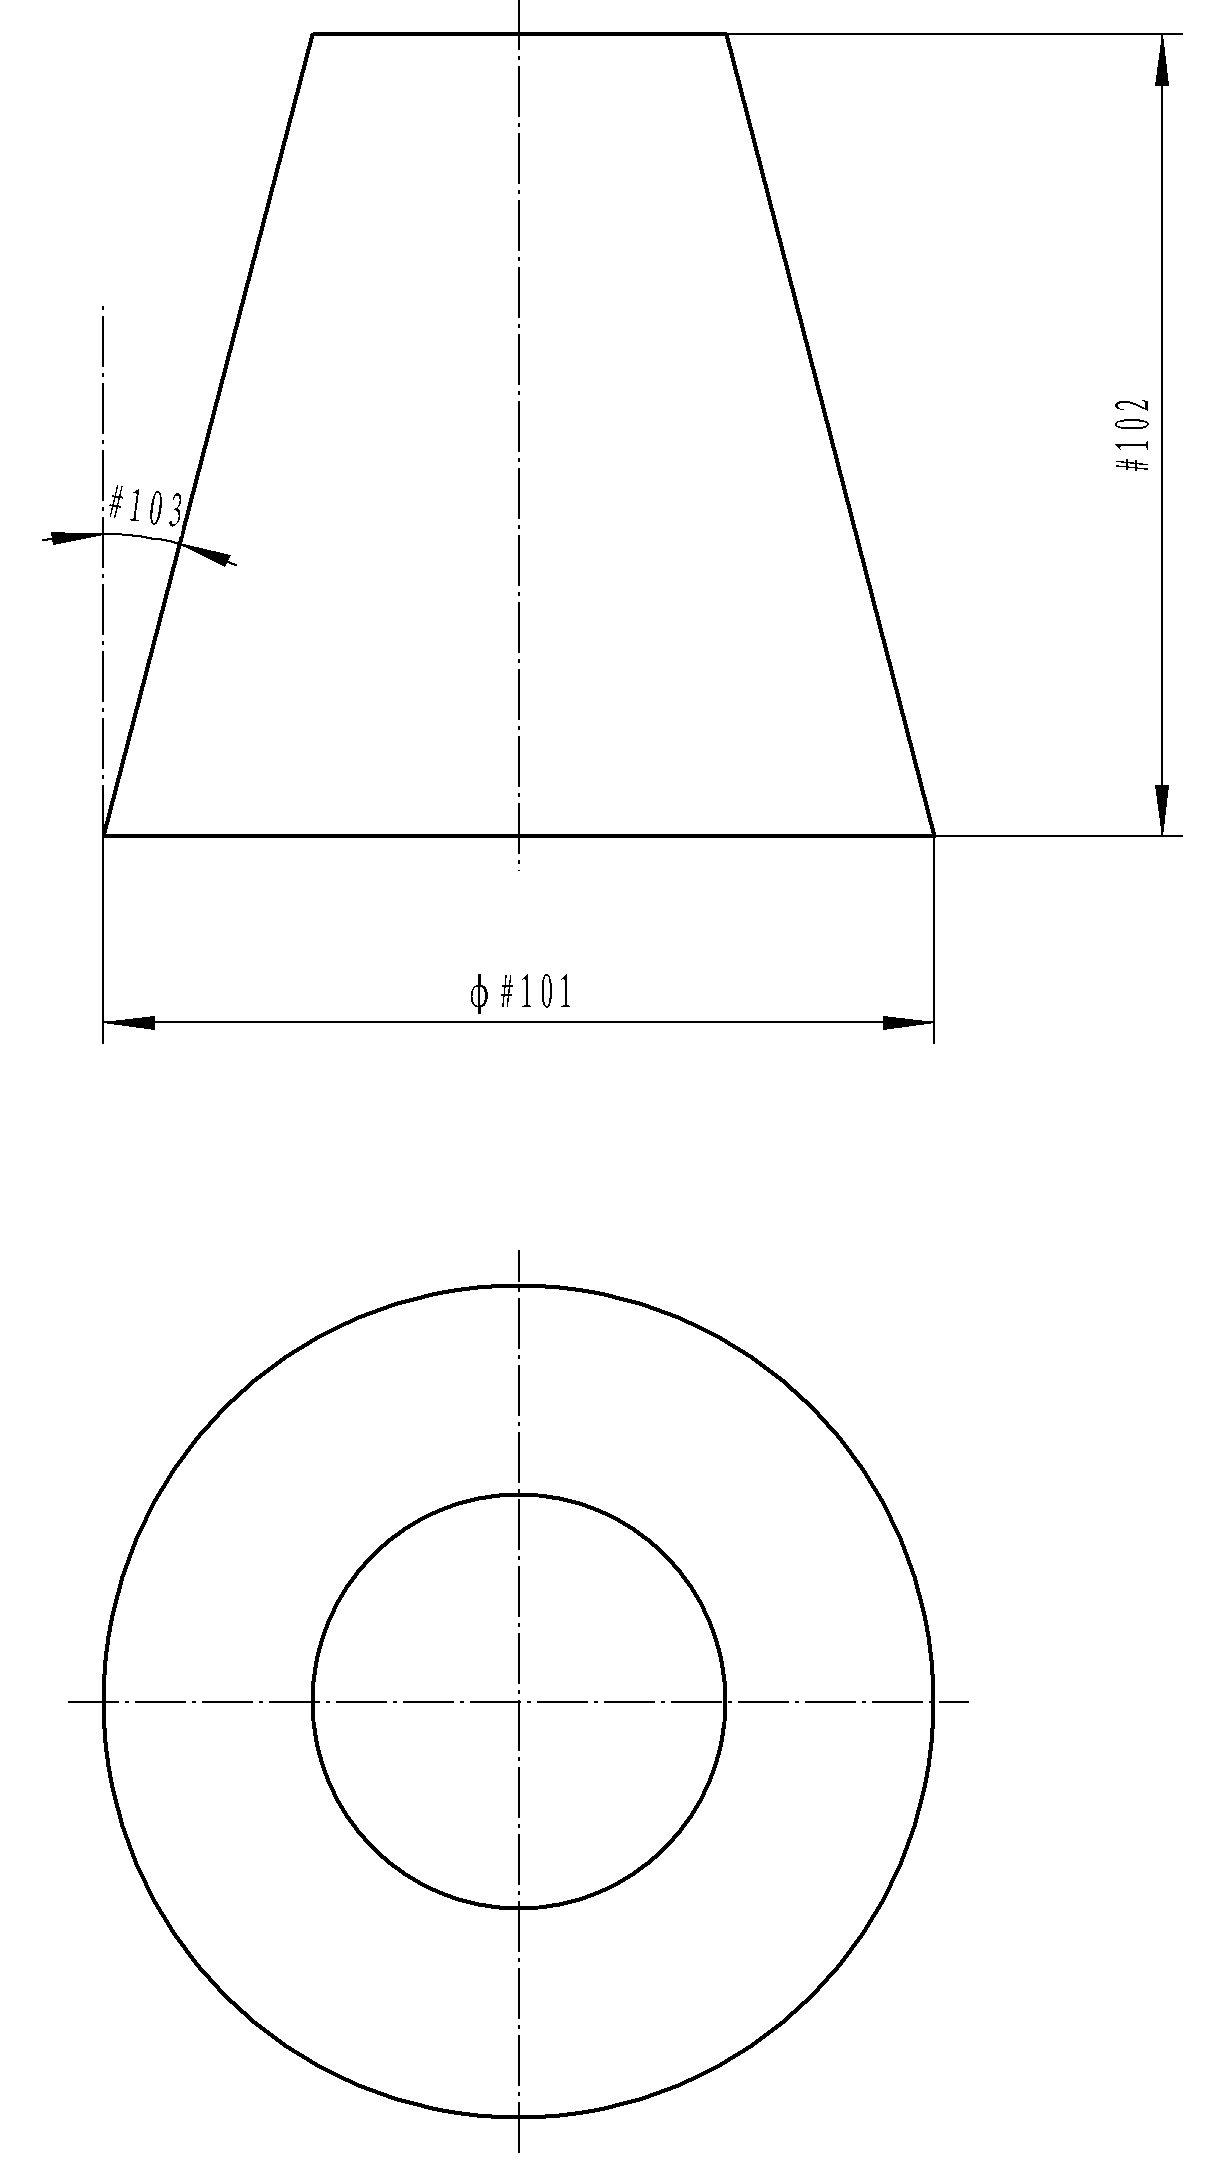
\includegraphics[width=0.4\textwidth]{images/13-1.jpg}
	\caption{圆锥} \label{圆锥}
\end{figure}
参考程序:
\begin{lstlisting}
O0001
#101=50
#102=20
#103=15
#104=8
#105=0.1
G54G17G40G49G90
M3S500
G1Z30.F2000
X-[#101/2+#104]Y0
Z5.0
Z-#102F200
#120=#102
WHILE[#120 GT 0]DO1
#120=#120-#105
G1Z-#120
#121=#101/2-[#102-#120]*TAN[#103]
X-[#121+#104] Y0
G2 I[#121+#104]
END1
G1 Z30.F2000
M5
M30
\end{lstlisting}
\subsubsection{写出如图\ref{圆角}所示零件的宏程序}
\begin{figure}
	\centering	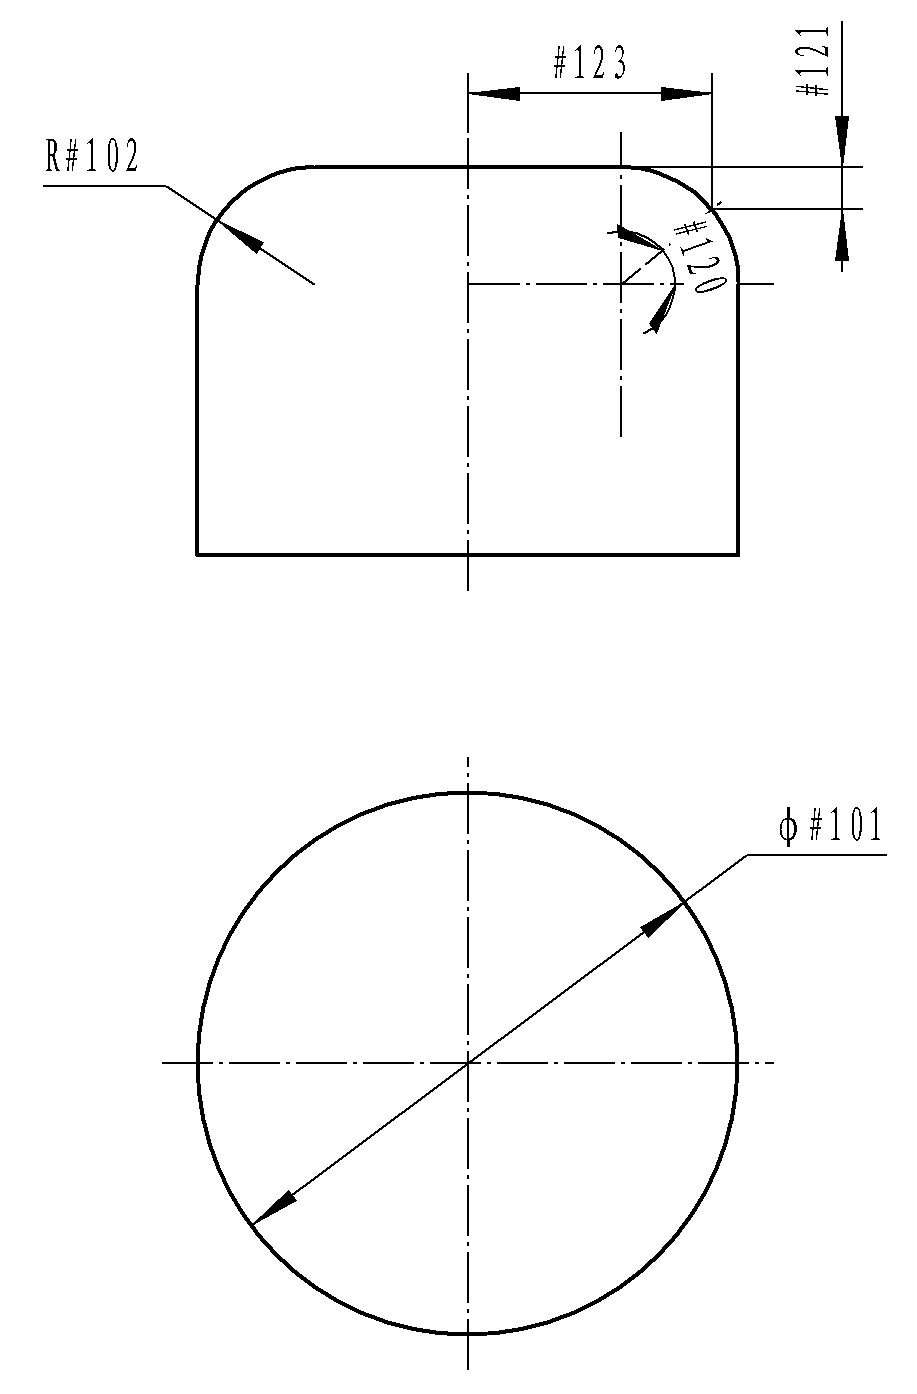
\includegraphics[width=0.4\textwidth]{images/13-2.jpg}
	\caption{圆角} \label{圆角}
\end{figure}
刀具半径: \#103

加工精度: \#104

Z向分层(用角度控制)

初始值: \#120=0

终止值: 90

\verb|#121=#102-#102*sin[#120]|

\verb|#122=#101/2-[#102-#102*cos[#120]]|

参考程序:
\begin{lstlisting}
O0001
#101----#104
G54G17G40G49G90
M3S500
G1Z30.F2000
X-[#101/2+#103+1]Y0
Z5.0
Z-#102F200
#120=0
WHILE[#120LT90]DO1
#120=#120+#104
#121=#102-#102*sin[#120]
G1Z-#121
#122=#101/2-[#102-#102*cos[#120]]
G1X-[#122+#103]Y0
G2I[#122+#103]
END1
G1Z30.F2000
M5
M30
\end{lstlisting}
\subsubsection{写出如图\ref{圆角:圆锥}所示零件的宏程序}:
\begin{figure}
	\centering	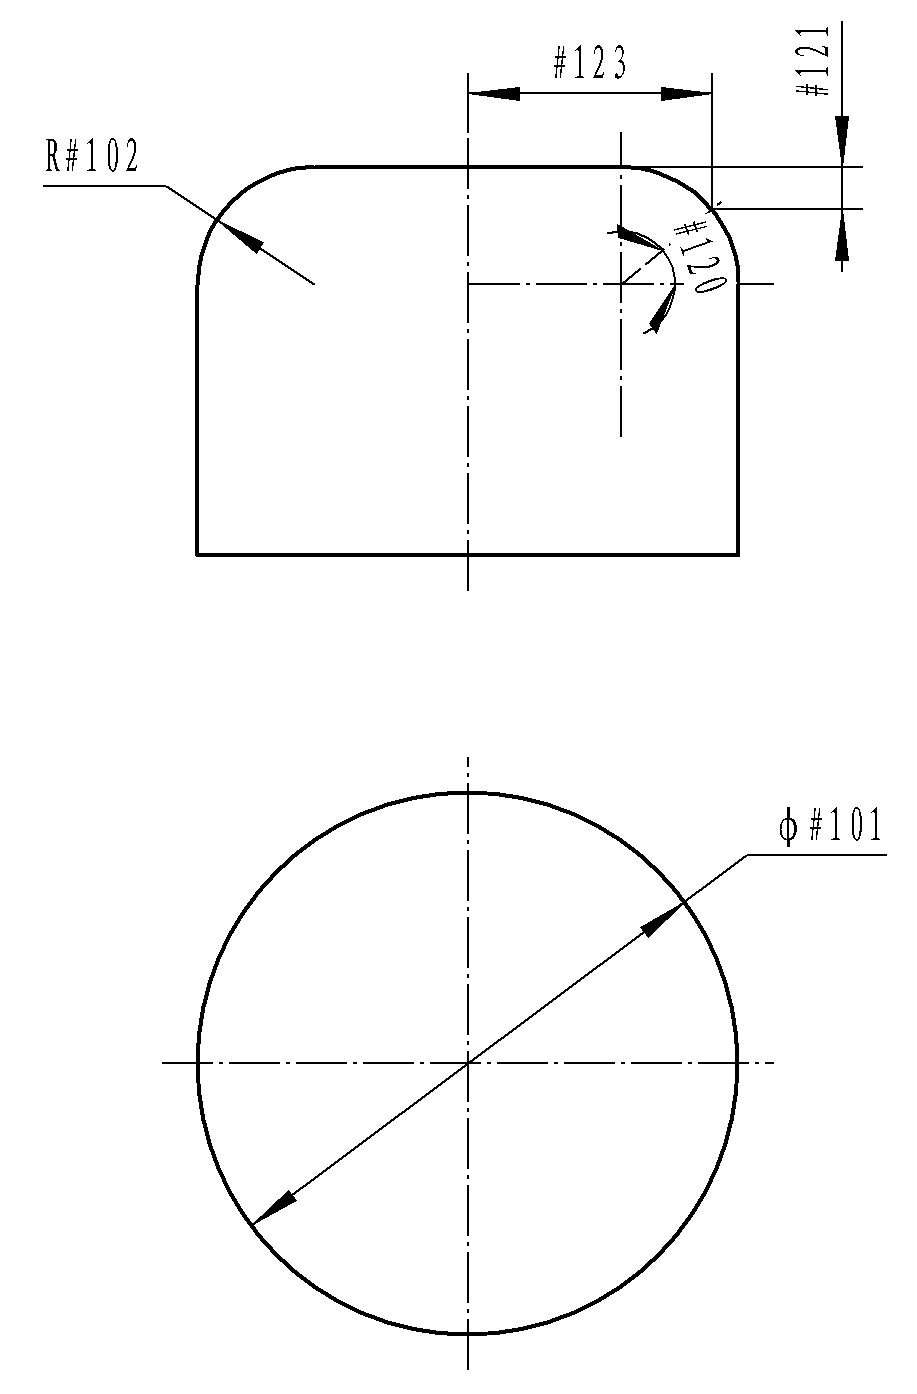
\includegraphics[width=0.4\textwidth]{images/13-2.jpg}
	\caption{圆角:圆锥} \label{圆角:圆锥}
\end{figure}
刀具:\#105

加工精度: \#106

角度精度: \#107

斜度:

Z向分层: 用长度控制

初始值: \#121=\#102

终止值为: \#102-\#131

\#131=\#102-\#103+\#103*SIN[\#104]

\#122=\#101-[\#102-\#121]*TAN[\#121]

圆角:

Z向分层:用角度控制

初始值: \#120=\#104

终止值: 90

\#121=\#103-\#103*sin[\#120]

\#122=\#132+\#103*cos[\#120]

\#132=\#103-\#131*tan[\#103]-\#102*cos[\#103]

参考程序:

\begin{lstlisting}
O0001
#101----#107
G54G17G40G49G90
M3S500
G1Z30.F2000
X-[#101+#105+2] Y0
Z5.0
Z-#102F200
#121=#102
#131=#102-#103+#103*SIN[#104]
WHILE[#121GT#131]DO1
#121=#121-#106
IF[#121LT#131]THEN#121=#131
G1Z-#121
#122=#101-[#102-#121]*TAN[#121]
X-[#122+#105]Y0
G2I[#122+#105]
END1
#132=#103-#131*tan[#103]-#102*cos[#103]
#120=#104
WHILE[#120LT90]DO1
#120=#120+#107
IF[#120GT90]THEN#120=90
#121=#103-#103*SIN[#120]
#122=#132+#103*COS[#120]
G1Z-#121
X-[#122+#105]Y0
G2I[#122+#105]
END1
G1Z30.F2000
M5
M30
\end{lstlisting}

\subsection{课堂小结}
\begin{enumerate}[1、]
	\item 简单零件的倒角;
	\item 宏程序实例1;
	\item 宏程序实例2。
\end{enumerate}

\vfill
\subsection{布置作业}
\begin{enumerate}[1、]
	\item 写出上面的程序;
	\item 从习题集上选做一个。
\end{enumerate}
\vfill